\section{Contexte}

Dans le développement logiciel moderne, la revue de code est devenue une pratique incontournable pour garantir la qualité et la maintenabilité des applications. Cette pratique consiste à examiner systématiquement le code source écrit par les développeurs avant son intégration dans la base de code principale. Au-delà de la simple détection de bugs, la revue de code favorise le partage de connaissances, l'uniformisation des pratiques de codage et l'apprentissage collectif au sein des équipes.

Avec l'adoption massive des méthodologies Agiles et DevOps, les cycles de développement se sont accélérés, multipliant ainsi le nombre de modifications de code à réviser. Les plateformes de gestion de versions comme GitHub et GitLab sont devenues centrales dans ce processus, offrant des outils intégrés pour faciliter les revues via les requêtes de fusion (Pull Requests (PR) / Merge Requests (MR)). Ces plateformes génèrent d'importantes quantités de données : commentaires, approbations, rejets, temps de révision, historiques de modifications, etc.

L’exploitation de ces données représente une opportunité majeure pour comprendre et optimiser les processus de développement. Dans le domaine de l’ingénierie logicielle empirique, les travaux de Mining Software Repositories montrent l’intérêt croissant de l’analyse des données issues des dépôts logiciels pour extraire des connaissances actionnables sur les projets et leurs processus \cite{vidoni2022systematic}. Dans un contexte DevOps, ces données permettent d’évaluer la performance des équipes, d’identifier les ralentissements dans le cycle de livraison et d’orienter les actions d’amélioration continue \cite{debellis2024dora,kudrjavets2024speed}. Elles sont également utilisées pour étudier la collaboration entre développeurs, la dynamique des revues de code et les risques associés aux changements proposés \cite{bacchelli2013expectations,gocmen2025enhanced}.

Cependant, l’accès à ces données et leur analyse restent problématiques. La collecte nécessite une connaissance approfondie des APIs des plateformes, une gestion complexe de l'authentification, de la pagination et des quotas de requêtes. De plus, les formats de données sont hétérogènes et nécessitent un traitement important avant toute analyse exploitable. Cette complexité technique constitue un frein majeur pour les chercheurs et les équipes souhaitant tirer parti de ces données.

\section{Présentation de l’organisme d’accueil et du cadre de collaboration}
Ce projet de fin d’études a été réalisé au sein de l’École nationale Supérieure d’Informatique d’Alger (ESI), en collaboration avec l’École de technologie supérieure de Montréal (ÉTS). Ce cadre de collaboration a permis d’associer un environnement de formation en ingénierie informatique à une expertise de recherche appliquée en génie logiciel.

L’École nationale Supérieure d’Informatique d’Alger est un établissement algérien spécialisé dans la formation supérieure en informatique. Créée en 1969 sous le nom de Centre d’Études et de Recherche en Informatique (CERI), elle est devenue l’Institut National de Formation en Informatique (INI) avant d’être transformée en École nationale supérieure en 2008. L’ESI assure notamment une formation d’ingénieur d’État en informatique sur cinq années, articulée autour d’un cycle préparatoire et d’un second cycle de spécialisation \cite{esiPresentation}.

L’École de technologie supérieure de Montréal est une université québécoise spécialisée en génie appliqué. Sa mission repose sur l’enseignement universitaire, la recherche appliquée et le transfert technologique, en lien étroit avec l’industrie. L’ÉTS occupe une place importante dans la formation en ingénierie au Québec, puisqu’elle forme une part significative des ingénieurs québécois et s’inscrit dans une dynamique d’innovation technologique \cite{etsAccueil}.

Dans ce contexte, le projet RevMine s’inscrit dans une collaboration académique entre l’ESI et l’ÉTS. La réalisation du projet a été encadrée côté ESI par notre encadrante académique, tandis que l’accompagnement scientifique côté ÉTS a été assuré par les promotrices associées au projet. Cette organisation a permis de bénéficier à la fois d’un suivi académique local et d’une expertise de recherche spécialisée dans l’analyse des processus logiciels et des données de revue de code.

La figure suivante illustre l’organisation de l’encadrement du projet RevMine. Elle met en évidence les étudiants porteurs du projet, l’encadrement assuré par l’ESI Alger ainsi que la collaboration scientifique avec l’ÉTS Montréal.


\begin{figure}[H]
\centering
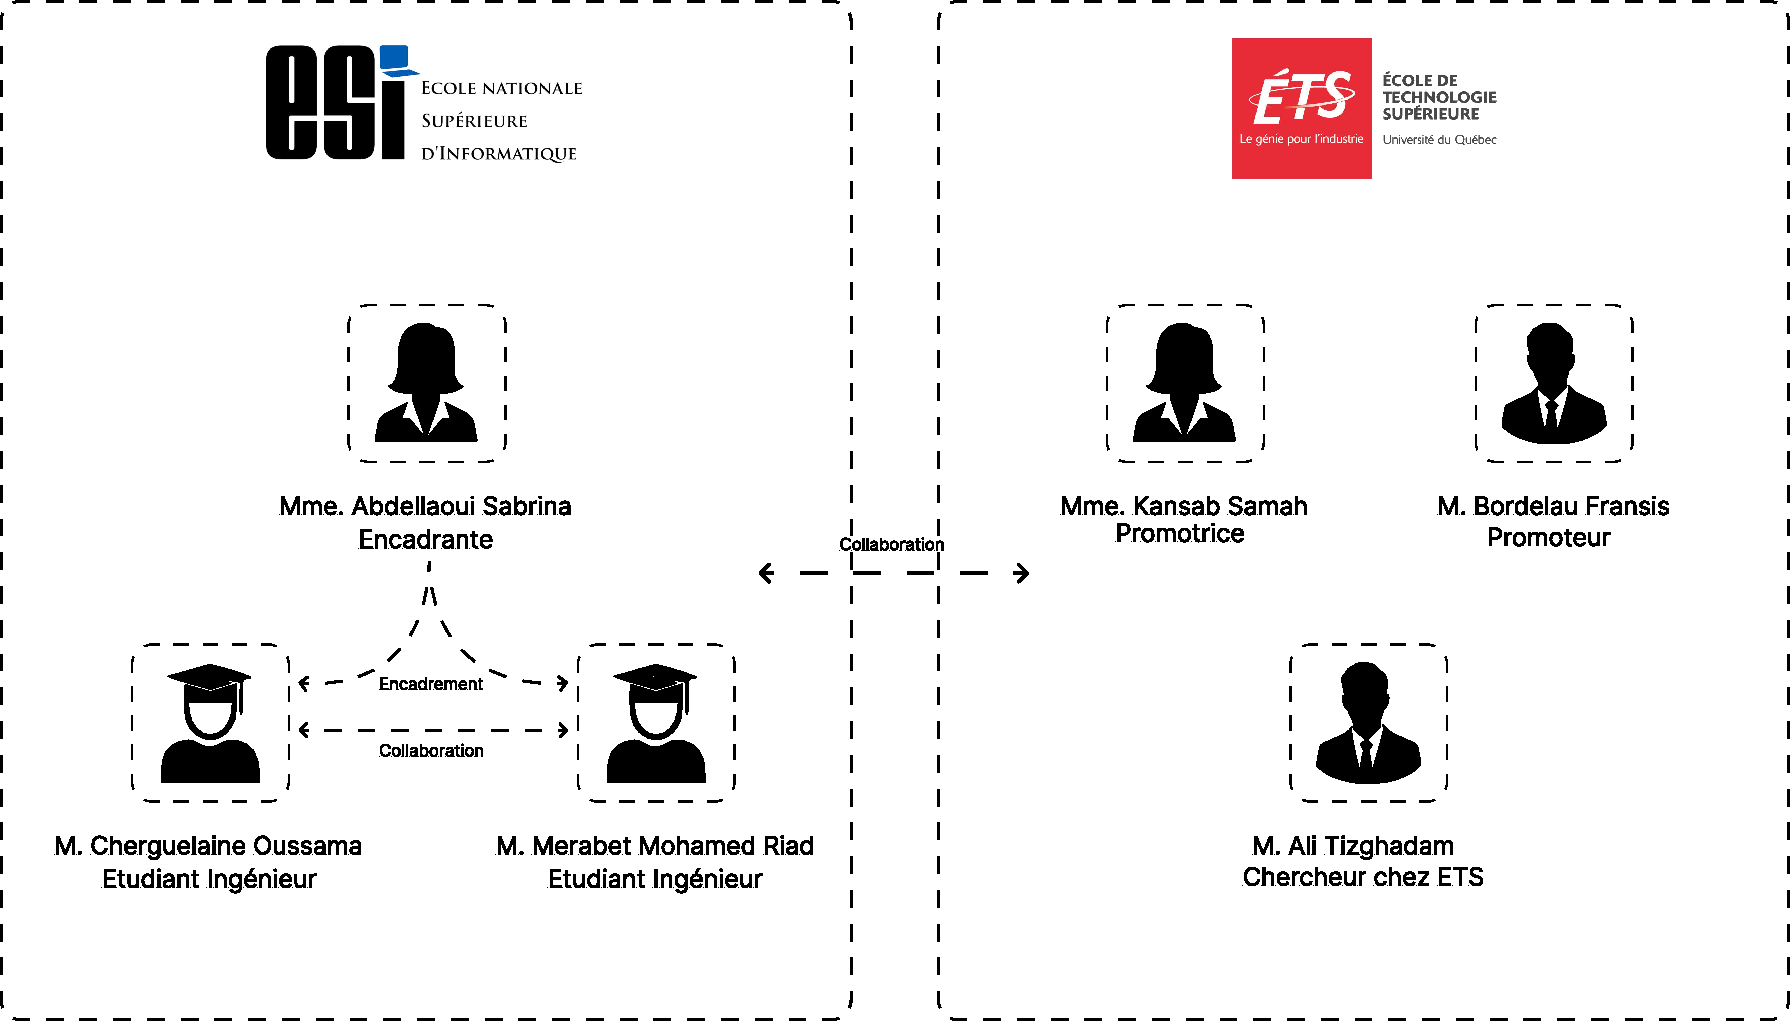
\includegraphics[width=0.9\textwidth]{figures/organisme_d_acceuil.pdf}
\caption{Organisation du projet RevMine}
\label{fig:encadrement-revmine}
\end{figure}


\section{Problématique}

Malgré l'importance croissante de la revue de code dans les pratiques DevOps et l'abondance de données générées par les plateformes comme GitHub et GitLab, plusieurs obstacles limitent leur exploitation efficace :

\begin{itemize}
     \item \textbf{Complexité de préparation de la collecte :}
    L’exploitation des données de revue de code ne se limite pas à l’appel des APIs. Elle nécessite un effort manuel important pour comprendre la structure des plateformes, sélectionner les bons points d’accès, gérer l’authentification, la pagination, les erreurs, les filtres de collecte et la normalisation des données. Cette phase de préparation impose souvent l’écriture de scripts spécifiques et rend le processus difficilement accessible aux utilisateurs non experts, en particulier lorsque l’objectif est de produire une collecte fiable et reproductible \cite{gousios2012ghtorrent,duenas2018perceval,vidoni2022systematic}.
    
    \item \textbf{Hétérogénéité des formats :} Les données provenant de différentes sources (GitHub, GitLab) présentent des structures et des formats variés, nécessitant des transformations et normalisations spécifiques.
    
    \item \textbf{Absence d'outils intégrés :} Il n'existe pas de solution unifiée permettant à la fois la collecte, le nettoyage, l'analyse et la visualisation des données de revue de code de manière accessible aux non-experts.
    
    \item \textbf{Barrière d'accessibilité :} Les chercheurs et praticiens qui ne possèdent pas de compétences avancées en programmation ou en manipulation d'APIs sont souvent exclus de ce type d'analyses.
    
    \item \textbf{Manque d'interactivité :} Les outils existants proposent généralement des analyses prédéfinies, sans permettre aux utilisateurs de formuler leurs propres questions ou d'explorer librement les données selon leurs besoins spécifiques.
\end{itemize}

Face à ces constats, la question centrale de ce projet est : \textbf{Comment faciliter l'accès, la collecte et l'analyse des données de revue de code pour les rendre exploitables par un large public, tout en offrant une interface intuitive et interactive ?}

\section{Objectifs}

Pour répondre à cette problématique, ce projet de fin d'études vise à développer \textbf{RevMine}, un outil interactif et accessible pour la collecte et l'analyse des données de revue de code. Les objectifs spécifiques sont les suivants :
\FloatBarrier
\begin{table}[h]
\centering
\caption{Objectifs du projet RevMine}
\label{tab:objectifs_smart}
\begin{tabular}{|c|p{0.8\textwidth}|}
\hline
\textbf{ID} & \textbf{Objectif} \\
\hline
\textbf{O1} & Réduire le temps de collecte de données de revue de code depuis GitHub et GitLab de 70\% en gérant l’authentification, la pagination et la normalisation. \\
\hline
\textbf{O2} & Développer une interface no-code accessible aux non-experts permettant la configuration complète sans programmation. \\
\hline
\textbf{O3} & Centraliser les phases de collecte, nettoyage, analyse et visualisation dans une plateforme unique, éliminant le besoin de recourir à 3-4 outils séparés. \\
\hline
\textbf{O4} & Intégrer un module LLM réduisant de 80\% le temps de personnalisation via requêtes en langage naturel et génération automatique d'analyses. \\
\hline
\textbf{O5} & Valider RevMine sur 3+ projets open source de tailles variées avec collecte réussie de plus de 90\% des données disponibles. \\
\hline
\textbf{O6} & Produire une documentation complète (installation, tutoriels, architecture) et un package de réplication open source. \\
\hline
\end{tabular}
\end{table}
\FloatBarrier
% \subsection{Objectif 1 : Collecte automatisée des données}

% Développer un module robuste capable de collecter automatiquement les données de revue de code à partir des APIs de GitHub et GitLab, en gérant :
% \begin{itemize}
%     \item L'authentification sécurisée
%     \item La pagination pour récupérer de grands volumes de données
%     \item Les quotas et limitations d'API
%     \item La gestion des erreurs et la reprise en cas d'échec
%     \item La normalisation des formats de données
% \end{itemize}

% \subsection{Objectif 2 : Interface utilisateur intuitive}

% Concevoir une interface graphique conviviale permettant :
% \begin{itemize}
%     \item La configuration facile des sources de données (dépôts, tokens d'accès)
%     \item Le suivi en temps réel de la progression de la collecte
%     \item L'exploration visuelle des données collectées
%     \item La sélection guidée des analyses à effectuer
% \end{itemize}

% \subsection{Objectif 3 : Intégration d'un module LLM pour les requêtes en langage naturel}

% Intégrer un modèle de langage (LLM) permettant aux utilisateurs de :
% \begin{itemize}
%     \item Formuler leurs questions d'analyse en langage naturel
%     \item Obtenir des réponses contextualisées basées sur les données collectées
%     \item Générer automatiquement des scripts d'analyse ou des visualisations
%     \item Bénéficier de suggestions d'analyses pertinentes
% \end{itemize}

% \subsection{Objectif 4 : Validation sur des projets open source}

% Valider l'outil sur plusieurs projets open source représentatifs pour :
% \begin{itemize}
%     \item Démontrer sa capacité à gérer différents types et tailles de projets
%     \item Collecter des datasets de référence utilisables par la communauté de recherche
%     \item Identifier et corriger les limitations de l'outil
%     \item Produire des analyses concrètes démontrant l'utilité de RevMine
% \end{itemize}

% \subsection{Objectif 5 : Documentation et reproductibilité}

% Fournir une documentation complète comprenant :
% \begin{itemize}
%     \item Un guide d'installation et de configuration
%     \item Des tutoriels d'utilisation avec exemples
%     \item Une documentation technique de l'architecture
%     \item Des exemples d'analyses reproductibles
% \end{itemize}

\section{Structure du mémoire}

Ce mémoire est structuré en deux grandes parties complémentaires, précédées d’une introduction générale et suivies d’une conclusion générale.

\textbf{Première partie : Étude bibliographique}

La première partie de ce mémoire présente les fondements théoriques et le contexte scientifique du projet RevMine. Elle vise à introduire les concepts essentiels liés à la revue de code, aux pratiques DevOps, à l’analyse des données logicielles, ainsi qu’à l’utilisation des modèles de langage (LLMs) dans l’ingénierie logicielle.

Le premier chapitre propose un état de l’art sur la revue de code et son rôle dans les pipelines DevOps modernes. Il aborde également les différentes approches d’analyse des données de développement logiciel ainsi que l’intégration des modèles de langage dans ces processus.

Le second chapitre est consacré à l’étude de l’existant. Il présente une analyse comparative des outils actuels de collecte et d’analyse des données issues des plateformes telles que GitHub et GitLab. Cette étude met en évidence les limites des solutions existantes et justifie la nécessité d’un outil comme RevMine.

\textbf{Deuxième partie : Contribution}

La deuxième partie de ce mémoire est dédiée à la contribution principale de ce projet, à savoir la conception, le développement et la validation de la plateforme RevMine.

Le premier chapitre de cette partie présente l’analyse des besoins, en identifiant les différents acteurs du système ainsi que les exigences fonctionnelles et non fonctionnelles auxquelles la plateforme doit répondre.

Le second chapitre décrit la conception de la solution proposée. Il détaille l’architecture générale du système, les différents modules, ainsi que les choix techniques et architecturaux adoptés.

Le troisième chapitre présente les métriques et les visualisations supportées par RevMine, en mettant en évidence leur intérêt pour l’analyse des processus de revue de code.

Le quatrième chapitre expose la réalisation de la plateforme. Il décrit les technologies utilisées, l’architecture microservices mise en place, ainsi que les différents composants développés, tant au niveau du backend que du frontend.

Enfin, un dernier chapitre est consacré à la validation et à l’évaluation de la solution proposée. Il présente les tests réalisés, les résultats obtenus ainsi que les limites du système.

Le mémoire se termine par une conclusion générale qui synthétise les contributions réalisées et propose des perspectives d’amélioration.